\documentclass{article}
\usepackage{graphicx}
\usepackage[spanish]{babel}
\usepackage{amsmath}

\begin{document}

\begin{titlepage}
    \centering
    \vspace*{2cm}
    
    {\Huge\bfseries Solución de Ejercicios del primer evento evaluativo\par}
    \vspace{1.5cm}
    
    {\Large\itshape Autor: Emanuel Cabrera Novoa\par}
    \vspace{1cm}
    
    {\large 13 de marzo de 2025\par}
    \vspace{2cm}
    
    
\includegraphics[width=0.4\textwidth]{media/Escudo_Universidad_de_Medellin.svg.png}
    \vfill
    
    {\large \textbf{Asignatura:} Química Orgánica\par}
    \vspace{0.5cm}
    
    {\large \textbf{Profesor:} Carlos Andrés Jiménes\par}
    \vspace{0.5cm}
    
    {\large \textbf{Universidad:} Universidad de Medellín\par}
    \vspace{1cm}
    
    \vfill
\end{titlepage}

\section{Solución punto 10}
Para nombrar cada uno de los ejemplos de los grupos funcionales se seguirán las normas dictadas por la IUPAC.

\subsection{Alcanos}
Para nombrar el siguiente alcano (ver Figura \ref{fig:alcano}) se siguen los siguientes pasos:
\begin{figure}[h]
    \centering
    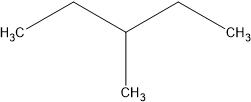
\includegraphics[width=0.5\linewidth]{media/3-metilpentano.jpg}
    \caption{Ejemplo de un alcano}
    \label{fig:alcano}
\end{figure}

\subsubsection{Identificar la cadena principal}
La cadena principal es la más larga de carbonos continuos. Si hay varias opciones con la misma cantidad de carbonos, se elige la que tenga más sustituyentes.

\subsubsection{Numerar la cadena principal}
Se enumera desde el extremo más cercano a un sustituyente. Si hay sustituyentes a igual distancia por ambos extremos, se elige la numeración que dé el menor número al primer sustituyente (ver Figura \ref{fig:numeracion_alcano}).
\begin{figure}[h]
    \centering
    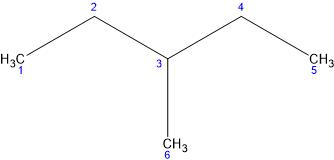
\includegraphics[width=0.5\linewidth]{media/numeracion 3-metilpentano.jpg}
    \caption{Numeración del alcano}
    \label{fig:numeracion_alcano}
\end{figure}

\subsubsection{Identificar y nombrar los sustituyentes}
Los sustituyentes se nombran como grupos alquilo (derivados de alcanos). Si hay varios sustituyentes iguales, se usan prefijos: \textbf{di-}, \textbf{tri-}, \textbf{tetra-}, etc.

\subsubsection{Indicar la posición de los sustituyentes}
Se usa el número del carbono al que están unidos. Los números se separan con comas (,) y de las palabras con guiones (-).

\subsubsection{Ordenar los sustituyentes alfabéticamente}
Se ignoran los prefijos \textit{di-}, \textit{tri-}, \textit{tetra-} al ordenar.

\subsubsection{Escribir el nombre final}
El formato es el siguiente: [posición]-[nombre del sustituyente][nombre de la cadena principal]. Si hay más de un sustituyente, se separan con comas y se escriben en orden alfabético.

\subsection{Alquenos}
Para nombrar el siguiente alqueno (ver Figura \ref{fig:alqueno}) se siguen los siguientes pasos:
\begin{figure}[h]
    \centering
    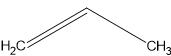
\includegraphics[width=0.5\linewidth]{media/propeno.jpg}
    \caption{Ejemplo de un alqueno}
    \label{fig:alqueno}
\end{figure}

\subsubsection{Identificar la cadena principal}
Se selecciona la cadena de carbonos más larga que contenga el doble enlace. Si hay dos o más cadenas de igual longitud, se elige la que tenga más enlaces dobles.

\subsubsection{Numerar la cadena principal}
La numeración debe empezar desde el extremo más cercano al doble enlace para asignarle el número más bajo posible. Si hay más de un doble enlace, se numera de manera que el primer doble enlace tenga el número más bajo.

\subsubsection{Nombrar la cadena principal}
Se usa la raíz del nombre del alcano correspondiente y se reemplaza la terminación ``-ano'' por ``-eno''. Si hay más de un doble enlace, se usan prefijos numéricos.

\subsubsection{Indicar la posición del doble enlace}
Se coloca el número del primer carbono del doble enlace antes del sufijo ``-eno''.

\subsubsection{Agregar sustituyentes (si hay)}
Se nombran en orden alfabético con sus respectivas posiciones en la cadena principal.

\subsection{Alquinos}
Para nombrar el siguiente alquino (ver Figura \ref{fig:alquino}) se siguen los siguientes pasos:
\begin{figure}[h]
    \centering
    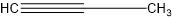
\includegraphics[width=0.5\linewidth]{media/propino.jpg}
    \caption{Ejemplo de un alquino}
    \label{fig:alquino}
\end{figure}

\subsubsection{Identificar la cadena principal}
Se selecciona la cadena de carbono más larga que contenga el triple enlace. Si hay dos cadenas con la misma cantidad de carbonos, se elige la que tenga más triples enlaces.

\subsubsection{Numerar la cadena principal}
Se numera desde el extremo más cercano al triple enlace para que tenga el número más bajo posible. Si hay más de un triple enlace, se numera de manera que el primero tenga el número más bajo.

\subsubsection{Nombrar la cadena principal}
Se usa la raíz del alcano correspondiente y se cambia la terminación ``-ano'' por ``-ino''. Si hay más de un triple enlace, se usan prefijos: -ino, -diino, -triino, etc.

\subsubsection{Indicar la posición del triple enlace}
Se coloca el número del primer carbono del triple enlace antes del sufijo ``-ino''.

\subsubsection{Agregar sustituyentes (si hay)}
Se nombran en orden alfabético con sus respectivas posiciones.

\subsection{Alcoholes}
Para nombrar el siguiente alcohol (ver Figura \ref{fig:alcohol}) se siguen los siguientes pasos:
\begin{figure}[h]
    \centering
    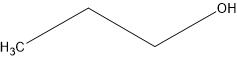
\includegraphics[width=0.5\linewidth]{media/propanol.jpg}
    \caption{Ejemplo de un alcohol}
    \label{fig:alcohol}
\end{figure}

\subsubsection{Identificar la cadena principal}
Se elige la cadena de carbonos más larga que contenga el grupo -OH.

\subsubsection{Numerar la cadena principal}
Se numera desde el extremo más cercano al grupo -OH, sin importar la ubicación de otros sustituyentes. El carbono al que está unido el grupo -OH debe recibir el número más bajo posible.

\subsubsection{Nombrar la cadena principal}
Se usa la raíz del nombre del alcano correspondiente y se cambia la terminación ``-o'' por ``-ol''. Si hay más de un grupo -OH, se usan prefijos: -ol, -diol, -triol, etc.

\subsubsection{Agregar sustituyentes (si hay)}
Se nombran en orden alfabético con sus respectivas posiciones en la cadena principal.

\subsection{Éteres}
Para nombrar el siguiente éter (ver Figura \ref{fig:eter}) se siguen los siguientes pasos:
\begin{figure}[h]
    \centering
    \includegraphics[width=0.5\linewidth]{media/dietiléter.jpg}
    \caption{Ejemplo de un éter}
    \label{fig:eter}
\end{figure}

\subsubsection{Identificar la cadena principal}
Se elige la cadena más larga como el hidrocarburo base (alcano principal).

\subsubsection{Nombrar el grupo -OR (alcoxi)}
La cadena más corta unida al oxígeno se nombra como un grupo ``alcóxi'' (derivado del alcano correspondiente, cambiando ``-ano'' por ``-oxi'').

\subsubsection{Numerar la cadena principal}
Se numera la cadena más larga de modo que el grupo -OR (alcóxi) tenga el número más bajo posible.

\subsubsection{Formar el nombre final}
Se escribe primero el nombre del grupo alcoxi, seguido del nombre del alcano principal.

\subsection{Aldehídos}
Para nombrar el siguiente aldehído (ver Figura \ref{fig:aldehido}) se siguen los siguientes pasos:
\begin{figure}[h]
    \centering
    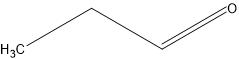
\includegraphics[width=0.5\linewidth]{media/propanal.jpg}
    \caption{Ejemplo de un aldehído}
    \label{fig:aldehido}
\end{figure}

\subsubsection{Identificar la cadena principal}
Se elige la cadena de carbonos más larga que incluya el grupo -CHO. Siempre se considera el carbono del grupo -CHO como C-1 (no es necesario numerarlo explícitamente).

\subsubsection{Nombrar la cadena principal}
Se usa el nombre del alcano correspondiente y se cambia la terminación ``-ano'' por ``-al''.

\subsubsection{Agregar sustituyentes (si hay)}
Se numeran los sustituyentes según la posición en la cadena, recordando que el carbono del grupo -CHO siempre es el C-1.

\subsection{Cetonas}
Para nombrar la siguiente cetona (ver Figura \ref{fig:cetona}) se siguen los siguientes pasos:
\begin{figure}[h]
    \centering
    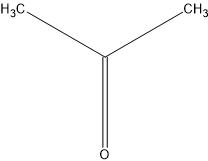
\includegraphics[width=0.5\linewidth]{media/propanona.jpg}
    \caption{Ejemplo de una cetona}
    \label{fig:cetona}
\end{figure}

\subsubsection{Nombrar la cadena principal}
Se usa el nombre del alcano correspondiente y se cambia la terminación ``-ano'' por ``-ona''. Se indica la posición del grupo carbonilo (C=O) con el número del carbono al que está unido.

\subsubsection{Agregar sustituyentes (si hay)}
Se nombran en orden alfabético con sus respectivas posiciones en la cadena principal.

\subsection{Ácidos Carboxílicos}
Para nombrar el siguiente ácido carboxílico (ver Figura \ref{fig:acido_carboxilico}) se siguen los siguientes pasos:
\begin{figure}[h]
    \centering
    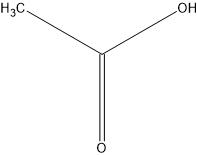
\includegraphics[width=0.5\linewidth]{media/ácido acético.jpg}
    \caption{Ejemplo de un ácido carboxílico}
    \label{fig:acido_carboxilico}
\end{figure}

\subsubsection{Nombrar la cadena principal}
Se usa el nombre del alcano correspondiente y se cambia la terminación ``-ano'' por ``-oico''. Siempre se antepone la palabra ``ácido''.

\subsubsection{Agregar sustituyentes (si hay)}
Se numeran los sustituyentes, recordando que el carbono del grupo -COOH siempre es el C-1.

\subsection{Ésteres}
Para nombrar el siguiente éster (ver Figura \ref{fig:ester}) se siguen los siguientes pasos:
\begin{figure}[h]
    \centering
    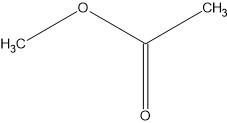
\includegraphics[width=0.5\linewidth]{media/etanoato de metilo.jpg}
    \caption{Ejemplo de un éster}
    \label{fig:ester}
\end{figure}

\subsubsection{Nombrar la parte del ácido carboxílico}
Se nombra el ácido carboxílico de origen, cambiando la terminación ``-oico'' por ``-oato''.

\subsubsection{Nombrar la parte del alcohol}
Se nombra el grupo alquilo derivado del alcohol y se escribe después de la parte del ácido.

\subsection{Aminas}
Para nombrar la siguiente amina (ver Figura \ref{fig:amina}) se siguen los siguientes pasos:
\begin{figure}[h]
    \centering
    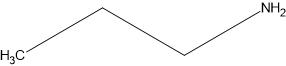
\includegraphics[width=0.5\linewidth]{media/propilamida.jpg}
    \caption{Ejemplo de una amina}
    \label{fig:amina}
\end{figure}

\subsubsection{Nombrar la cadena principal}
Se usa el nombre del alcano correspondiente y se cambia la terminación ``-o'' por ``-amina''. Si hay más de un grupo amino, se indican con los prefijos \textit{di-}, \textit{tri-}, etc.

\subsubsection{Numerar la cadena principal}
Se numera la cadena de modo que el grupo -NH2 tenga el número más bajo posible.

\subsection{Amidas}
Para nombrar la siguiente amida (ver Figura \ref{fig:amida}) se siguen los siguientes pasos:
\begin{figure}[h]
    \centering
    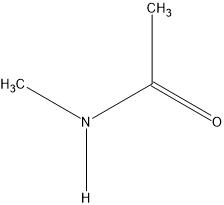
\includegraphics[width=0.5\linewidth]{media/metil etil amida.jpg}
    \caption{Ejemplo de una amida}
    \label{fig:amida}
\end{figure}

\subsubsection{Nombrar la cadena principal}
Se usa el nombre del ácido carboxílico correspondiente, cambiando la terminación ``-oico'' por ``-amida''.

\subsubsection{Nombrar los sustituyentes en el nitrógeno}
Si hay grupos alquilo unidos al nitrógeno, se indican con la letra ``N-'' seguida del nombre del alquilo.

\section{Solución punto 5}

\subsection{Hibridación \( sp^3 \) del Metano (\( \text{CH}_4 \))}

\subsubsection{Configuración electrónica del carbono}
El carbono (C) tiene un número atómico \( Z = 6 \), por lo que su configuración electrónica en el estado fundamental es:
\[
\text{C}: 1s^2 \, 2s^2 \, 2p^2
\]
- Tiene 4 electrones de valencia (2 en el orbital \( 2s \) y 2 en los orbitales \( 2p \)).

\subsubsection{Promoción de un electrón}
Para formar 4 enlaces, el carbono promueve uno de sus electrones del orbital \( 2s \) al orbital \( 2p \) vacío. Esto requiere energía, pero se compensa con la formación de enlaces más fuertes. La configuración electrónica del carbono en estado excitado es:
\[
\text{C}^*: 1s^2 \, 2s^1 \, 2p^3
\]
- Ahora tiene 4 electrones desapareados disponibles para formar enlaces.

\subsubsection{Hibridación \( sp^3 \)}
El carbono combina su orbital \( 2s \) y los tres orbitales \( 2p \) (\( 2p_x \), \( 2p_y \), \( 2p_z \)) para formar \textbf{4 orbitales híbridos \( sp^3 \)}. Estos orbitales híbridos son equivalentes en energía y forma.

- \textbf{Forma de los orbitales \( sp^3 \)}:
  - Cada orbital \( sp^3 \) tiene un lóbulo grande y uno pequeño.
  - Están orientados hacia los vértices de un \textbf{tetraedro}, con ángulos de \( 109.5^\circ \) entre ellos.

\subsubsection{Formación de enlaces en el metano}
En el metano (\( \text{CH}_4 \)):
\begin{enumerate}
    \item Cada uno de los 4 orbitales \( sp^3 \) del carbono se superpone con el orbital \( 1s \) de un átomo de hidrógeno (H).
    \item Esta superposición forma \textbf{4 enlaces sigma (\( \sigma \))}, que son enlaces covalentes fuertes.
    \item La geometría resultante es \textbf{tetraédrica}, con el carbono en el centro y los 4 hidrógenos en los vértices.
\end{enumerate}

\subsubsection{Geometría tetraédrica}
La geometría tetraédrica es el resultado de la repulsión entre los pares de electrones de los enlaces. Los 4 orbitales \( sp^3 \) se orientan lo más lejos posible entre sí para minimizar la repulsión, lo que da lugar a ángulos de enlace de \( 109.5^\circ \).

\subsubsection{Estructura del metano}
La estructura del metano se puede representar de la siguiente manera:

\begin{figure}
    \centering
    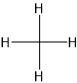
\includegraphics[width=0.5\linewidth]{media/metano.jpg}
    \caption{Metano}
    \label{fig:metano}
\end{figure}

- El carbono está en el centro.
- Los 4 hidrógenos están en los vértices de un tetraedro.

\subsubsection{Resumen de la hibridación \( sp^3 \)}
\begin{table}[h!]
\centering
\begin{tabular}{|c|c|}
\hline
\textbf{Característica} & \textbf{Descripción} \\
\hline
Orbitales involucrados & 1 orbital \( 2s \) + 3 orbitales \( 2p \) (\( 2p_x \), \( 2p_y \), \( 2p_z \)) \\
\hline
Número de orbitales \( sp^3 \) & 4 orbitales híbridos equivalentes \\
\hline
Geometría & Tetraédrica \\
\hline
Ángulos de enlace & \( 109.5^\circ \) \\
\hline
Ejemplo & Metano (\( \text{CH}_4 \)) \\
\hline
\end{tabular}
\end{table}


\subsection{Hibridación \( sp^2 \) del Etileno (\( \text{C}_2\text{H}_4 \))}

\subsubsection{Configuración electrónica del carbono}
El carbono (C) tiene un número atómico \( Z = 6 \), por lo que su configuración electrónica en el estado fundamental es:
\[
\text{C}: 1s^2 \, 2s^2 \, 2p^2
\]
- Tiene 4 electrones de valencia (2 en el orbital \( 2s \) y 2 en los orbitales \( 2p \)).

\subsubsection{Promoción de un electrón}
Para formar 3 enlaces sigma (\( \sigma \)) y 1 enlace pi (\( \pi \)), cada carbono promueve uno de sus electrones del orbital \( 2s \) al orbital \( 2p \) vacío. La configuración electrónica del carbono en estado excitado es:
\[
\text{C}^*: 1s^2 \, 2s^1 \, 2p^3
\]
- Ahora tiene 4 electrones desapareados disponibles para formar enlaces.

\subsubsection{Hibridación \( sp^2 \)}
Cada carbono combina su orbital \( 2s \) y dos de los orbitales \( 2p \) (\( 2p_x \), \( 2p_y \)) para formar \textbf{3 orbitales híbridos \( sp^2 \)}. El orbital \( 2p_z \) restante no se hibrida y permanece sin cambios.

- \textbf{Forma de los orbitales \( sp^2 \)}:
  - Cada orbital \( sp^2 \) tiene un lóbulo grande y uno pequeño.
  - Están orientados en un plano, con ángulos de \( 120^\circ \) entre ellos (geometría plana trigonal).

\subsubsection{Formación de enlaces en el etileno}
En el etileno (\( \text{C}_2\text{H}_4 \)):
\begin{enumerate}
    \item Cada carbono usa 2 de sus orbitales \( sp^2 \) para formar enlaces sigma (\( \sigma \)) con los átomos de hidrógeno (H).
    \item El tercer orbital \( sp^2 \) de cada carbono se superpone con el orbital \( sp^2 \) del otro carbono, formando un enlace sigma (\( \sigma \)) entre los dos carbonos.
    \item Los orbitales \( 2p_z \) no hibridados de cada carbono se superponen lateralmente para formar un enlace pi (\( \pi \)).
    \item La geometría resultante es \textbf{plana trigonal}, con ángulos de enlace de \( 120^\circ \).
\end{enumerate}

\subsubsection{Geometría plana trigonal}
La geometría plana trigonal es el resultado de la repulsión entre los pares de electrones de los enlaces. Los 3 orbitales \( sp^2 \) se orientan en un plano, lo que da lugar a ángulos de enlace de \( 120^\circ \).

\subsubsection{Estructura del etileno}
La estructura del etileno se puede representar de la siguiente manera:

\begin{figure}[h]
    \centering
    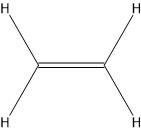
\includegraphics[width=0.5\linewidth]{media/etileno.jpg}
    \caption{Estructura del etileno}
    \label{fig:etileno}
\end{figure}

- Los dos carbonos están unidos por un doble enlace (1 enlace sigma y 1 enlace pi).
- Cada carbono está unido a 2 hidrógenos.

\subsubsection{Resumen de la hibridación \( sp^2 \)}
\begin{table}[h!]
\centering
\begin{tabular}{|c|c|}
\hline
\textbf{Característica} & \textbf{Descripción} \\
\hline
Orbitales involucrados & 1 orbital \( 2s \) + 2 orbitales \( 2p \) (\( 2p_x \), \( 2p_y \)) \\
\hline
Número de orbitales \( sp^2 \) & 3 orbitales híbridos equivalentes \\
\hline
Geometría & Plana trigonal \\
\hline
Ángulos de enlace & \( 120^\circ \) \\
\hline
Ejemplo & Etileno (\( \text{C}_2\text{H}_4 \)) \\
\hline
\end{tabular}
\end{table}

\subsection{Hibridación \( sp \) del Acetileno (\( \text{C}_2\text{H}_2 \))}

\subsubsection{Configuración electrónica del carbono}
El carbono (C) tiene un número atómico \( Z = 6 \), por lo que su configuración electrónica en el estado fundamental es:
\[
\text{C}: 1s^2 \, 2s^2 \, 2p^2
\]
- Tiene 4 electrones de valencia (2 en el orbital \( 2s \) y 2 en los orbitales \( 2p \)).

\subsubsection{Promoción de un electrón}
Para formar 2 enlaces sigma (\( \sigma \)) y 2 enlaces pi (\( \pi \)), cada carbono promueve uno de sus electrones del orbital \( 2s \) al orbital \( 2p \) vacío. La configuración electrónica del carbono en estado excitado es:
\[
\text{C}^*: 1s^2 \, 2s^1 \, 2p^3
\]
- Ahora tiene 4 electrones desapareados disponibles para formar enlaces.

\subsubsection{Hibridación \( sp \)}
Cada carbono combina su orbital \( 2s \) y uno de los orbitales \( 2p \) (\( 2p_x \)) para formar \textbf{2 orbitales híbridos \( sp \)}. Los orbitales \( 2p_y \) y \( 2p_z \) restantes no se hibridan y permanecen sin cambios.

- \textbf{Forma de los orbitales \( sp \)}:
  - Cada orbital \( sp \) tiene un lóbulo grande y uno pequeño.
  - Están orientados en línea recta, con un ángulo de \( 180^\circ \) entre ellos (geometría lineal).

\subsubsection{Formación de enlaces en el acetileno}
En el acetileno (\( \text{C}_2\text{H}_2 \)):
\begin{enumerate}
    \item Cada carbono usa 1 de sus orbitales \( sp \) para formar un enlace sigma (\( \sigma \)) con un átomo de hidrógeno (H).
    \item El segundo orbital \( sp \) de cada carbono se superpone con el orbital \( sp \) del otro carbono, formando un enlace sigma (\( \sigma \)) entre los dos carbonos.
    \item Los orbitales \( 2p_y \) y \( 2p_z \) no hibridados de cada carbono se superponen lateralmente para formar dos enlaces pi (\( \pi \)).
    \item La geometría resultante es \textbf{lineal}, con ángulos de enlace de \( 180^\circ \).
\end{enumerate}

\subsubsection{Geometría lineal}
La geometría lineal es el resultado de la repulsión entre los pares de electrones de los enlaces. Los 2 orbitales \( sp \) se orientan en línea recta, lo que da lugar a ángulos de enlace de \( 180^\circ \).

\subsubsection{Estructura del acetileno}
La estructura del acetileno se puede representar de la siguiente manera:

\begin{figure}[h]
    \centering
    \includegraphics[width=0.5\linewidth]{media/acetileno.png}
    \caption{acetileno}
    \label{fig:acetileno}
\end{figure}

- Los dos carbonos están unidos por un triple enlace (1 enlace sigma y 2 enlaces pi).
- Cada carbono está unido a 1 hidrógeno.

\subsection*{7. Resumen de la hibridación \( sp \)}
\begin{table}[h!]
\centering
\begin{tabular}{|c|c|}
\hline
\textbf{Característica} & \textbf{Descripción} \\
\hline
Orbitales involucrados & 1 orbital \( 2s \) + 1 orbital \( 2p \) (\( 2p_x \)) \\
\hline
Número de orbitales \( sp \) & 2 orbitales híbridos equivalentes \\
\hline
Geometría & Lineal \\
\hline
Ángulos de enlace & \( 180^\circ \) \\
\hline
Ejemplo & Acetileno (\( \text{C}_2\text{H}_2 \)) \\
\hline
\end{tabular}
\end{table}

\end{document}
